%%% Local Variables:
%%% mode: latex
%%% Tex-engine: XeLaTeX
%%% TeX-master: t
%%% End:

\documentclass{article}

\usepackage{fancyhdr}
\usepackage{extramarks}
\usepackage{amsmath,amsthm,amssymb,amsthm}
\usepackage{enumitem}
\usepackage{tikz}
\usepackage[plain]{algorithm}
\usepackage{algpseudocode}
\usepackage[utf8]{inputenc}
\usepackage{color,soul}
\usepackage{graphicx}
\usepackage{minted}
\usepackage[english]{babel}

\graphicspath{ {./} }

\usetikzlibrary{automata,positioning}

%
% Basic Document Settings
%

\topmargin=-0.45in
\evensidemargin=0in
\oddsidemargin=0in
\textwidth=6.5in
\textheight=9.0in
\headsep=0.25in

\linespread{1.1}

\pagestyle{fancy}
%%\lhead{\hmwkAuthorName}
\chead{\hmwkClass\: \hmwkTitle}
\rhead{\firstxmark}
\lfoot{\lastxmark}
\cfoot{\thepage}

\renewcommand\headrulewidth{0.4pt}
\renewcommand\footrulewidth{0.4pt}

\setlength\parindent{0pt}

%
% Create Problem Sections
%

\newcommand{\enterProblemHeader}[1]{
    \nobreak\extramarks{}{Problem \arabic{#1} continued on next page\ldots}\nobreak{}
    \nobreak\extramarks{Problem \arabic{#1} (continued)}{Problem \arabic{#1} continued on next page\ldots}\nobreak{}
}

\newcommand{\exitProblemHeader}[1]{
    \nobreak\extramarks{Problem \arabic{#1} (cont.)}{Problem \arabic{#1} continued on next page\ldots}\nobreak{}
    \stepcounter{#1}
    \nobreak\extramarks{Problem \arabic{#1}}{}\nobreak{}
}

\setcounter{secnumdepth}{0}
\newcounter{partCounter}
\newcounter{homeworkProblemCounter}
\setcounter{homeworkProblemCounter}{1}
\nobreak\extramarks{Problem \arabic{homeworkProblemCounter}}{}\nobreak{}

%
% Homework Problem Environment
%
% This environment takes an optional argument. When given, it will adjust the
% problem counter. This is useful for when the problems given for your
% assignment aren't sequential. See the last 3 problems of this template for an
% example.
%
\newenvironment{homeworkProblem}[1][-1]{
    \ifnum#1>0
        \setcounter{homeworkProblemCounter}{#1}
    \fi
    
    \section{Problem \arabic{homeworkProblemCounter}}
    \setcounter{partCounter}{1}
    \enterProblemHeader{homeworkProblemCounter}
}{
    \exitProblemHeader{homeworkProblemCounter}
}

%
% Homework Details
%   - Title
%   - Due date
%   - Class
%   - Section/Time
%   - Instructor
%   - Author
%

\newcommand{\hmwkTitle}{Assignment \#1}
\newcommand{\hmwkDueDate}{September 19th, 2018}
\newcommand{\hmwkClass}{COMP 524 - Cybersecurity}
\newcommand{\hmwkClassInstructor}{Dr. Michael Soltys}
\newcommand{\hmwkAuthorName}{
  Rihan Stephen Pereira\\
  \text{email - rihanstephen.pereira576@myci.csuci.edu, studentID - 002497665}
  \\
  David Bryne\\
  \texttt{email - david.byrne@myci.csuci.edu}
  \\
  Marco Cabrera\\
  \text{email - marco.cabrera561@myci.csuci.edu, studentID - 002456715}
  \\
  Kaveh Arashvand\\
  \texttt{email - kaveh.arashvand075@myci.csuci.edu, studentID - 002377350}
}
%
% Title Page
%

\title{
    \vspace{2in}
    \textmd{\textbf{\hmwkClass:\ \hmwkTitle}}\\
    \normalsize\vspace{0.1in}\small{Due\ on\ \hmwkDueDate}\\
    \vspace{0.1in}\large{\textit{\hmwkClassInstructor\ \hmwkClassTime}}
    \vspace{3in}
}

\author{\hmwkAuthorName}

\renewcommand{\part}[1]{\textbf{\large Part \Alph{partCounter}}\stepcounter{partCounter}\\}

%
% Various Helper Commands
%

% Useful for algorithms
\newcommand{\alg}[1]{\textsc{\bfseries \footnotesize #1}}

% For derivatives
\newcommand{\deriv}[1]{\frac{\mathrm{d}}{\mathrm{d}x} (#1)}

% For partial derivatives
\newcommand{\pderiv}[2]{\frac{\partial}{\partial #1} (#2)}

% Integral dx
\newcommand{\dx}{\mathrm{d}x}

% Alias for the Solution section header
\newcommand{\solution}{\textbf{\large Solution}}

\newcommand{\justif}[2]{&{#1}&\text{#2}}

% Probability commands: Expectation, Variance, Covariance, Bias
\newcommand{\E}{\mathrm{E}}
\newcommand{\Var}{\mathrm{Var}}
\newcommand{\Cov}{\mathrm{Cov}}
\newcommand{\Bias}{\mathrm{Bias}}
\newcommand{\contradiction}{
  \ensuremath{{\Rightarrow\mspace{-2mu}\Leftarrow}}
}

% latex code for generating python code snippets
% Default fixed font does not support bold face
\DeclareFixedFont{\ttb}{T1}{txtt}{bx}{n}{12} % for bold
\DeclareFixedFont{\ttm}{T1}{txtt}{m}{n}{12}  % for normal

% Custom colors
\usepackage{color}
\definecolor{deepblue}{rgb}{0,0,0.5}
\definecolor{deepred}{rgb}{0.6,0,0}
\definecolor{deepgreen}{rgb}{0,0.5,0}

\usepackage{listings}

% Python style for highlighting
\newcommand\pythonstyle{\lstset{
language=Python,
basicstyle=\ttm,
otherkeywords={self},             % Add keywords here
keywordstyle=\ttb\color{deepblue},
emph={MyClass,__init__},          % Custom highlighting
emphstyle=\ttb\color{deepred},    % Custom highlighting style
stringstyle=\color{deepgreen},
frame=tb,                         % Any extra options here
showstringspaces=false            % 
}}


% Python environment
\lstnewenvironment{python}[1][]
{
\pythonstyle
\lstset{#1}
}
{}

% Python for external files
\newcommand\pythonexternal[2][]{{
\pythonstyle
\lstinputlisting[#1]{#2}}}

% Python for inline
\newcommand\pythoninline[1]{{\pythonstyle\lstinline!#1!}}
% end py code snippets

\begin{document}
\maketitle
\pagebreak

% problem 1
\begin{homeworkProblem}
  Decrypt the following four documents. To submit the assignment, write a two page PDF report, which explains, with code snippets, how you managed to decrypt the documents, and what the documents were.
  \begin{itemize}
    \item \textcolor{cyan}{\ul{assignment-1-a.txt}}: Caesar cipher Base64 encoded text
    \item \textcolor{cyan}{\ul{assignment-1-b.txt}}: MAC cipher Base64 encoded text
    \item \textcolor{cyan}{\ul{assignment-1-c.txt}}: Caesar cipher Base64 encoded jpeg
    \item \textcolor{cyan}{\ul{assignment-1-d.txt}}: MAC cipher Base64 encoded jpeg
  \end{itemize}
  \\
  \textbf{Solution:}
  \\
  \textbf{Caesar cipher Base64 encoded text}
  \\
  File - \textcolor{cyan}{\ul{assignment-1-a.txt}}
  \\
  \\
  A brute-force approach was used to solve this problem. From one of the three basic classical attacks, we applied \textit{Ciphertext only attack}, also called as \textit{recognizable plaintext attack}. Considering we are dealing with Caesar Cipher(CC) base64 encrypted text, we were sure that its using one of the 63 possible keys from 64 character alphabet list to encrypt the plaintext. From Dr. soltys notes, we used decryption function

  \begin{align*}
    D_n(x) &= (x + n) (mod 64)
  \end{align*}

  Also, we ignored keys $n = 0$ and  $n = 64$, since the obtained ciphertext is same as plaintext. Each key was used to break the cipher followed by base64 decoding on the decrypted text to get the plaintext. On offset 19 i.e key $n = 19$, we got the plaintext. It is a poem from \textit{William Blake}.
  \\
  \\
  Python code snippet we used to obtain plaintext:
  \pythonexternal{cc_plaintext_decrypt.py}
  \\
  \\
  The below images shows the plaintext that we obtained after running the above code fragment.
  \begin{figure}[h!]
    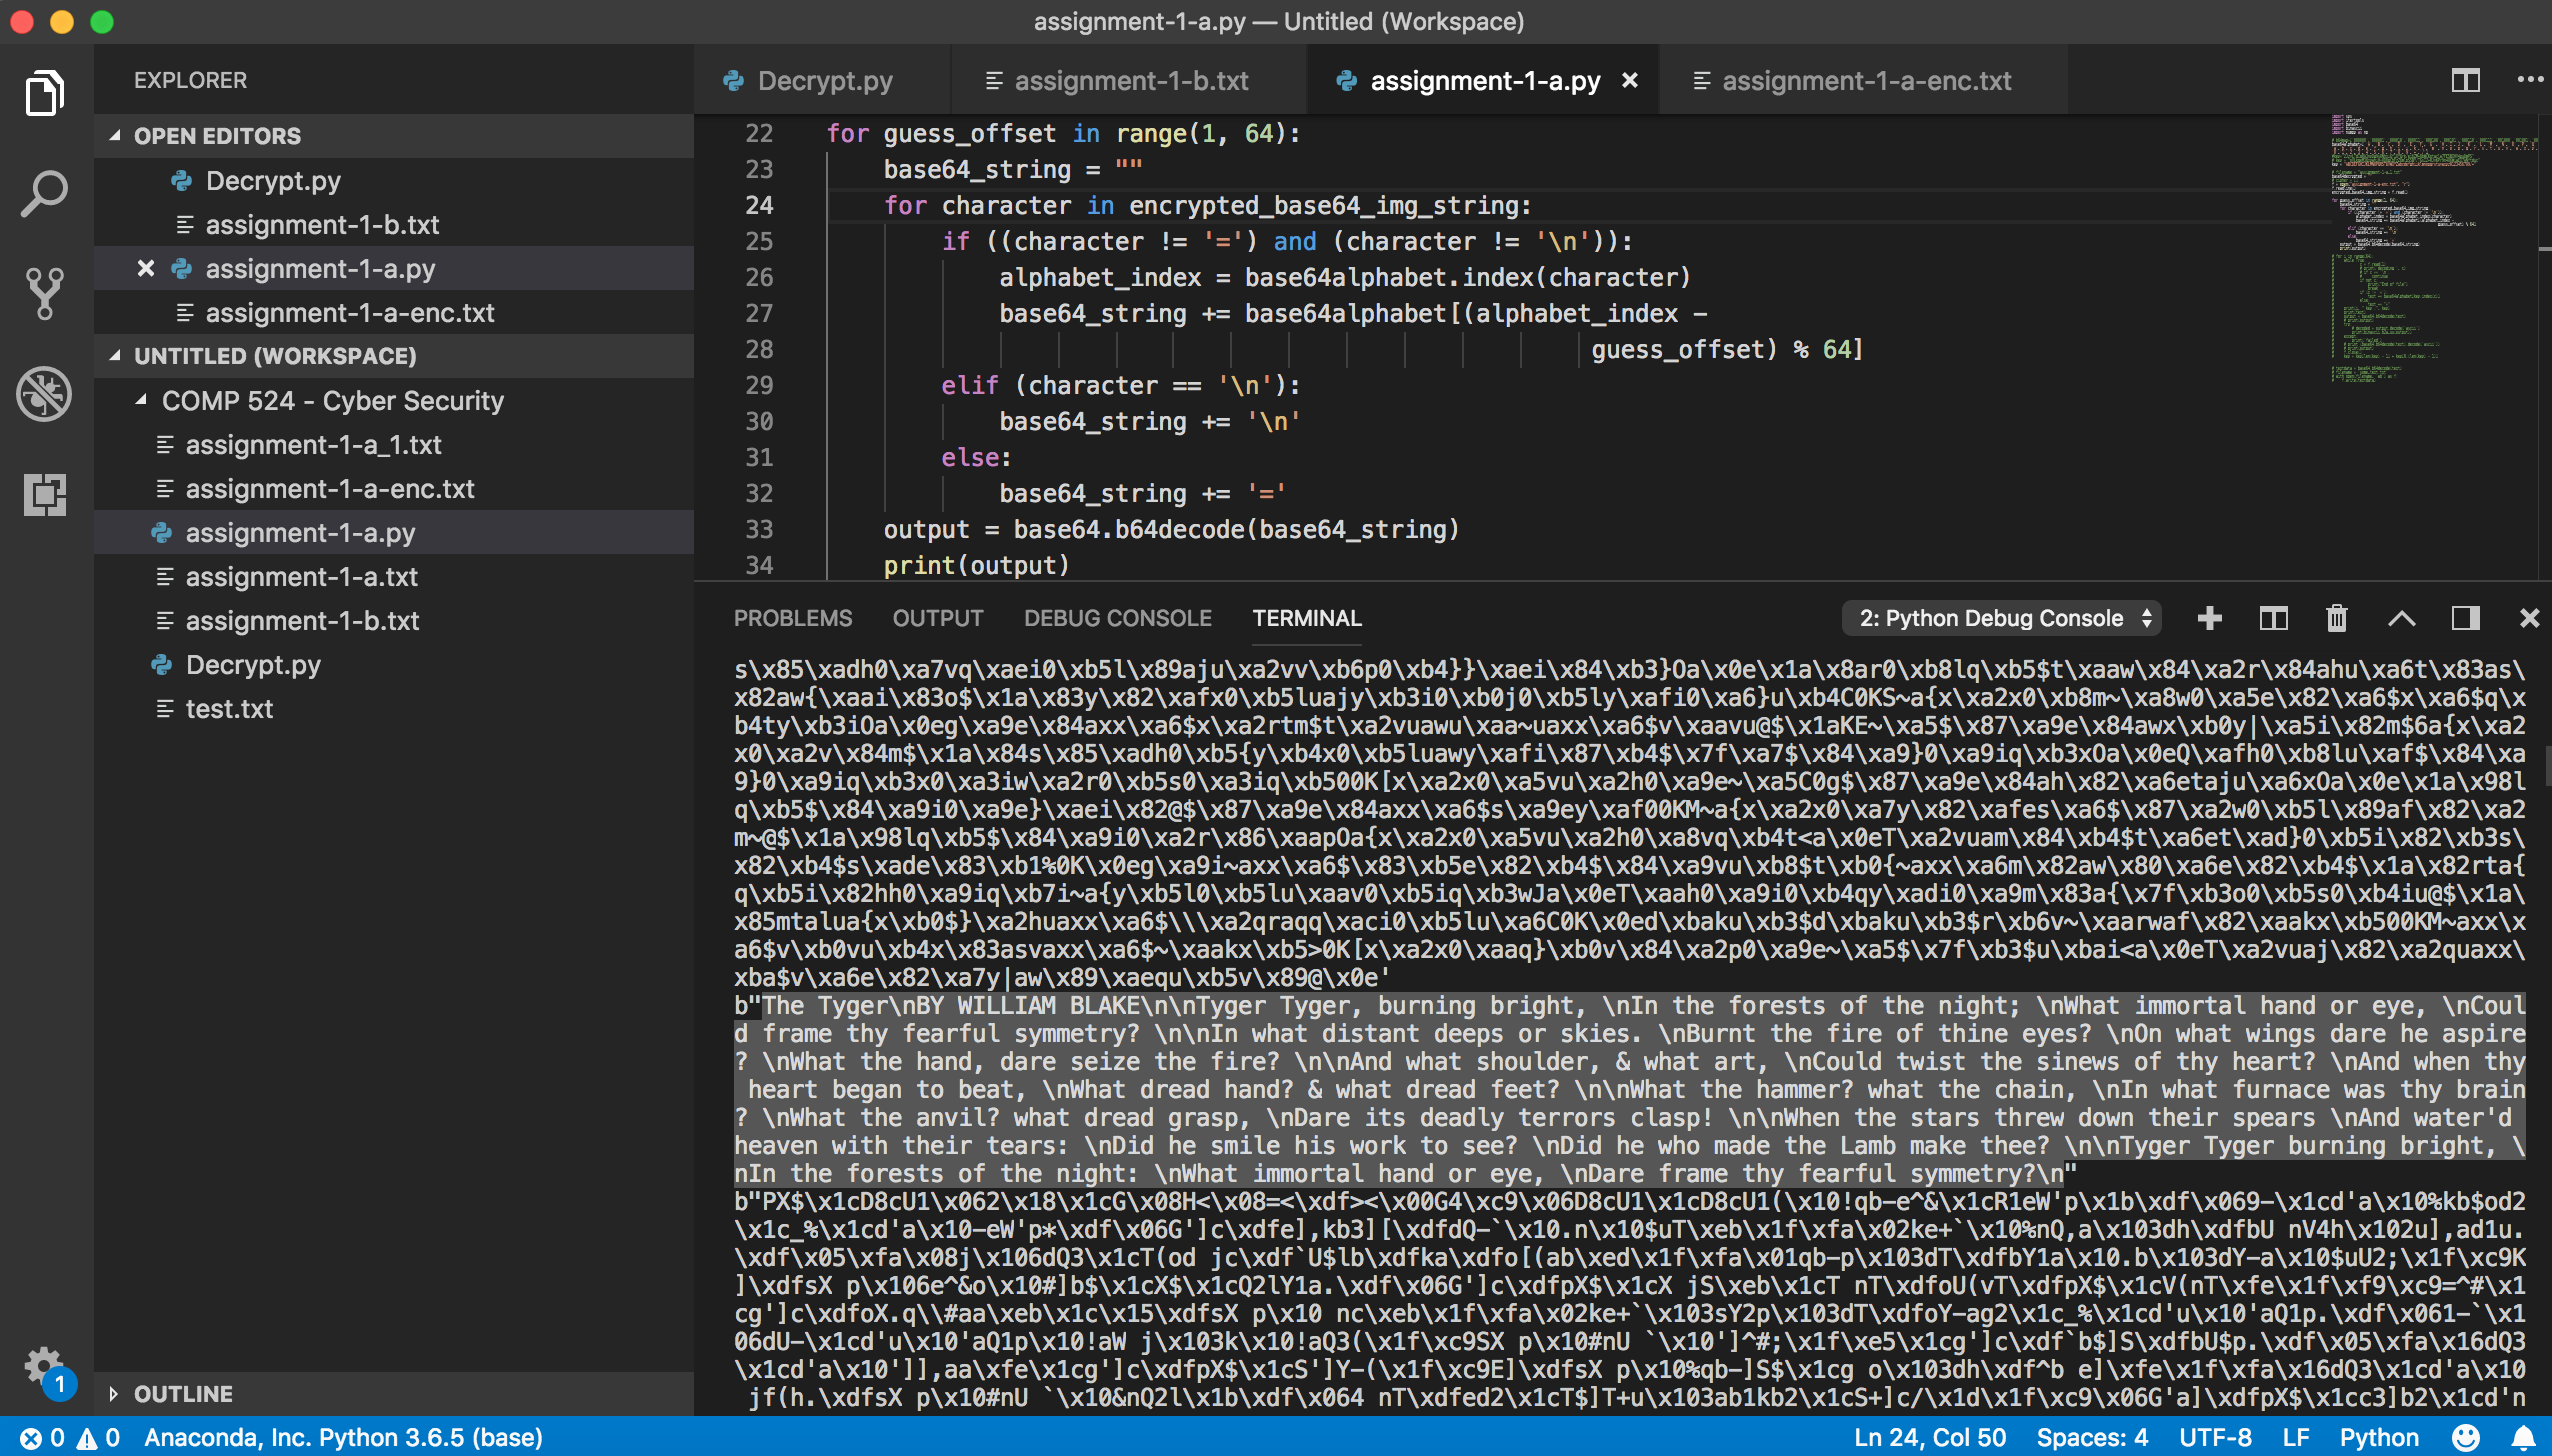
\includegraphics[width=18cm,height=13cm,keepaspectratio]{assign_1_output.png}
    \caption{assignment-1-a.txt deciphered and decoded output}
  \end{figure}

\end{homeworkProblem}

\pagebreak

% problem 1b
\begin{homeworkProblem}
\\
\textbf{MAC cipher Base64 encoded text}
\\
File - \textcolor{cyan}{\ul{assignment-1-b.txt}}
\\
\end{homeworkProblem}

\pagebreak

% problem 1c
\begin{homeworkProblem}
\\
\textbf{Caesar cipher Base64 encoded image}
\\
File - \textcolor{cyan}{\ul{assignment-1-c.txt}}
\\
To crack this secret, we used \textit{recognizable plaintext attack}, also called \textit{Ciphertext only} attack. We performed brute force on the ciphertext - scanning all the keys and for each key we used the Decryption function 

\begin{align*}
  D_n(x) &= (x + n) (mod 64)
\end{align*}
where, $x$ is the character from ciphertext and $n$ is the key for that iteration. Also, note that the key $n = 0$ or $n = 64$ were not considered because it doesn't not change the original plaintext. For each key, after running the decryption function, base64 decoding was applied to the text, and that base64 data was saved to disk as an image. Doing this, we saved altogether 
63 images to the disk. Finally, we found key $n = 9$ was used to encrypt the plaintext which gave us the resulting image during decryption.
\\
\\
Python code snippet for decrypting and decoding Caesar Cipher base64 jpeg:
\pythonexternal{decrypt_cc_images.py}
\\
\begin{figure}[h!]
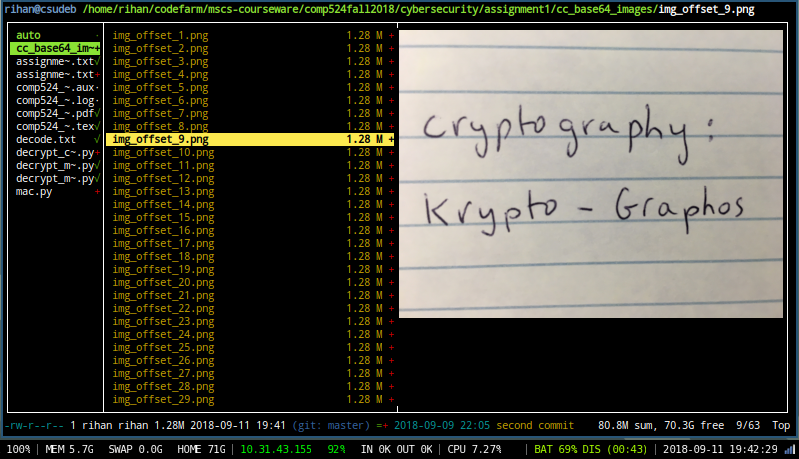
\includegraphics[width=18cm,height=10cm,keepaspectratio]{cc_image_cipher_detected_cli.png}
\caption{assignment-1-c.txt Caesar cipher decrypted and decoded image}
\end{figure}
\end{homeworkProblem}

\pagebreak

% problem 1d
\begin{homeworkProblem}
  \\
  \textbf{MAC cipher Base64 encoded jpeg}
  \\
  File - \textcolor{cyan}{\ul{assignment-1-d.txt}}
  \\
  \\
  The approach I used to solve this problem was a known text attack. By inspecting the other image that was decoded in problem 3 I was able to determine the header and byte offset that was included when the image was taken from an iphone. Then after we base64 encoded that known image I was able to count the exact offset of the header in base64 characters. Once I had this offset decrypting the key was just a matter of comparing the character at the same offset in both the encrypted file and the know file. Once we had a mapping for every character we were able to write a python script that decrypted and decoded the file. 
  \\
  The tool I used to calculate the byte offset of the image header was 0xd
  \\
  \\
  The key is: \ul{2JzvLTdIARk3nyDg9s0NhxjGf18YQrq/ei6ZM+ObWCKotaclw7FE5BXHV4puUmPS}
  \\
  \\
  The python program solution\_1d.py will output the decrypted image to a file. You can run this code: python solution\_1d.py
  \\
  \\
  Here is the Python code snippet which uses above key to reveal the secret jpeg image.
  \pythonexternal{solution_1d.py}
  \\
  The jpeg image secret that we found after breaking the ciphertext:
  \begin{figure}[h!]   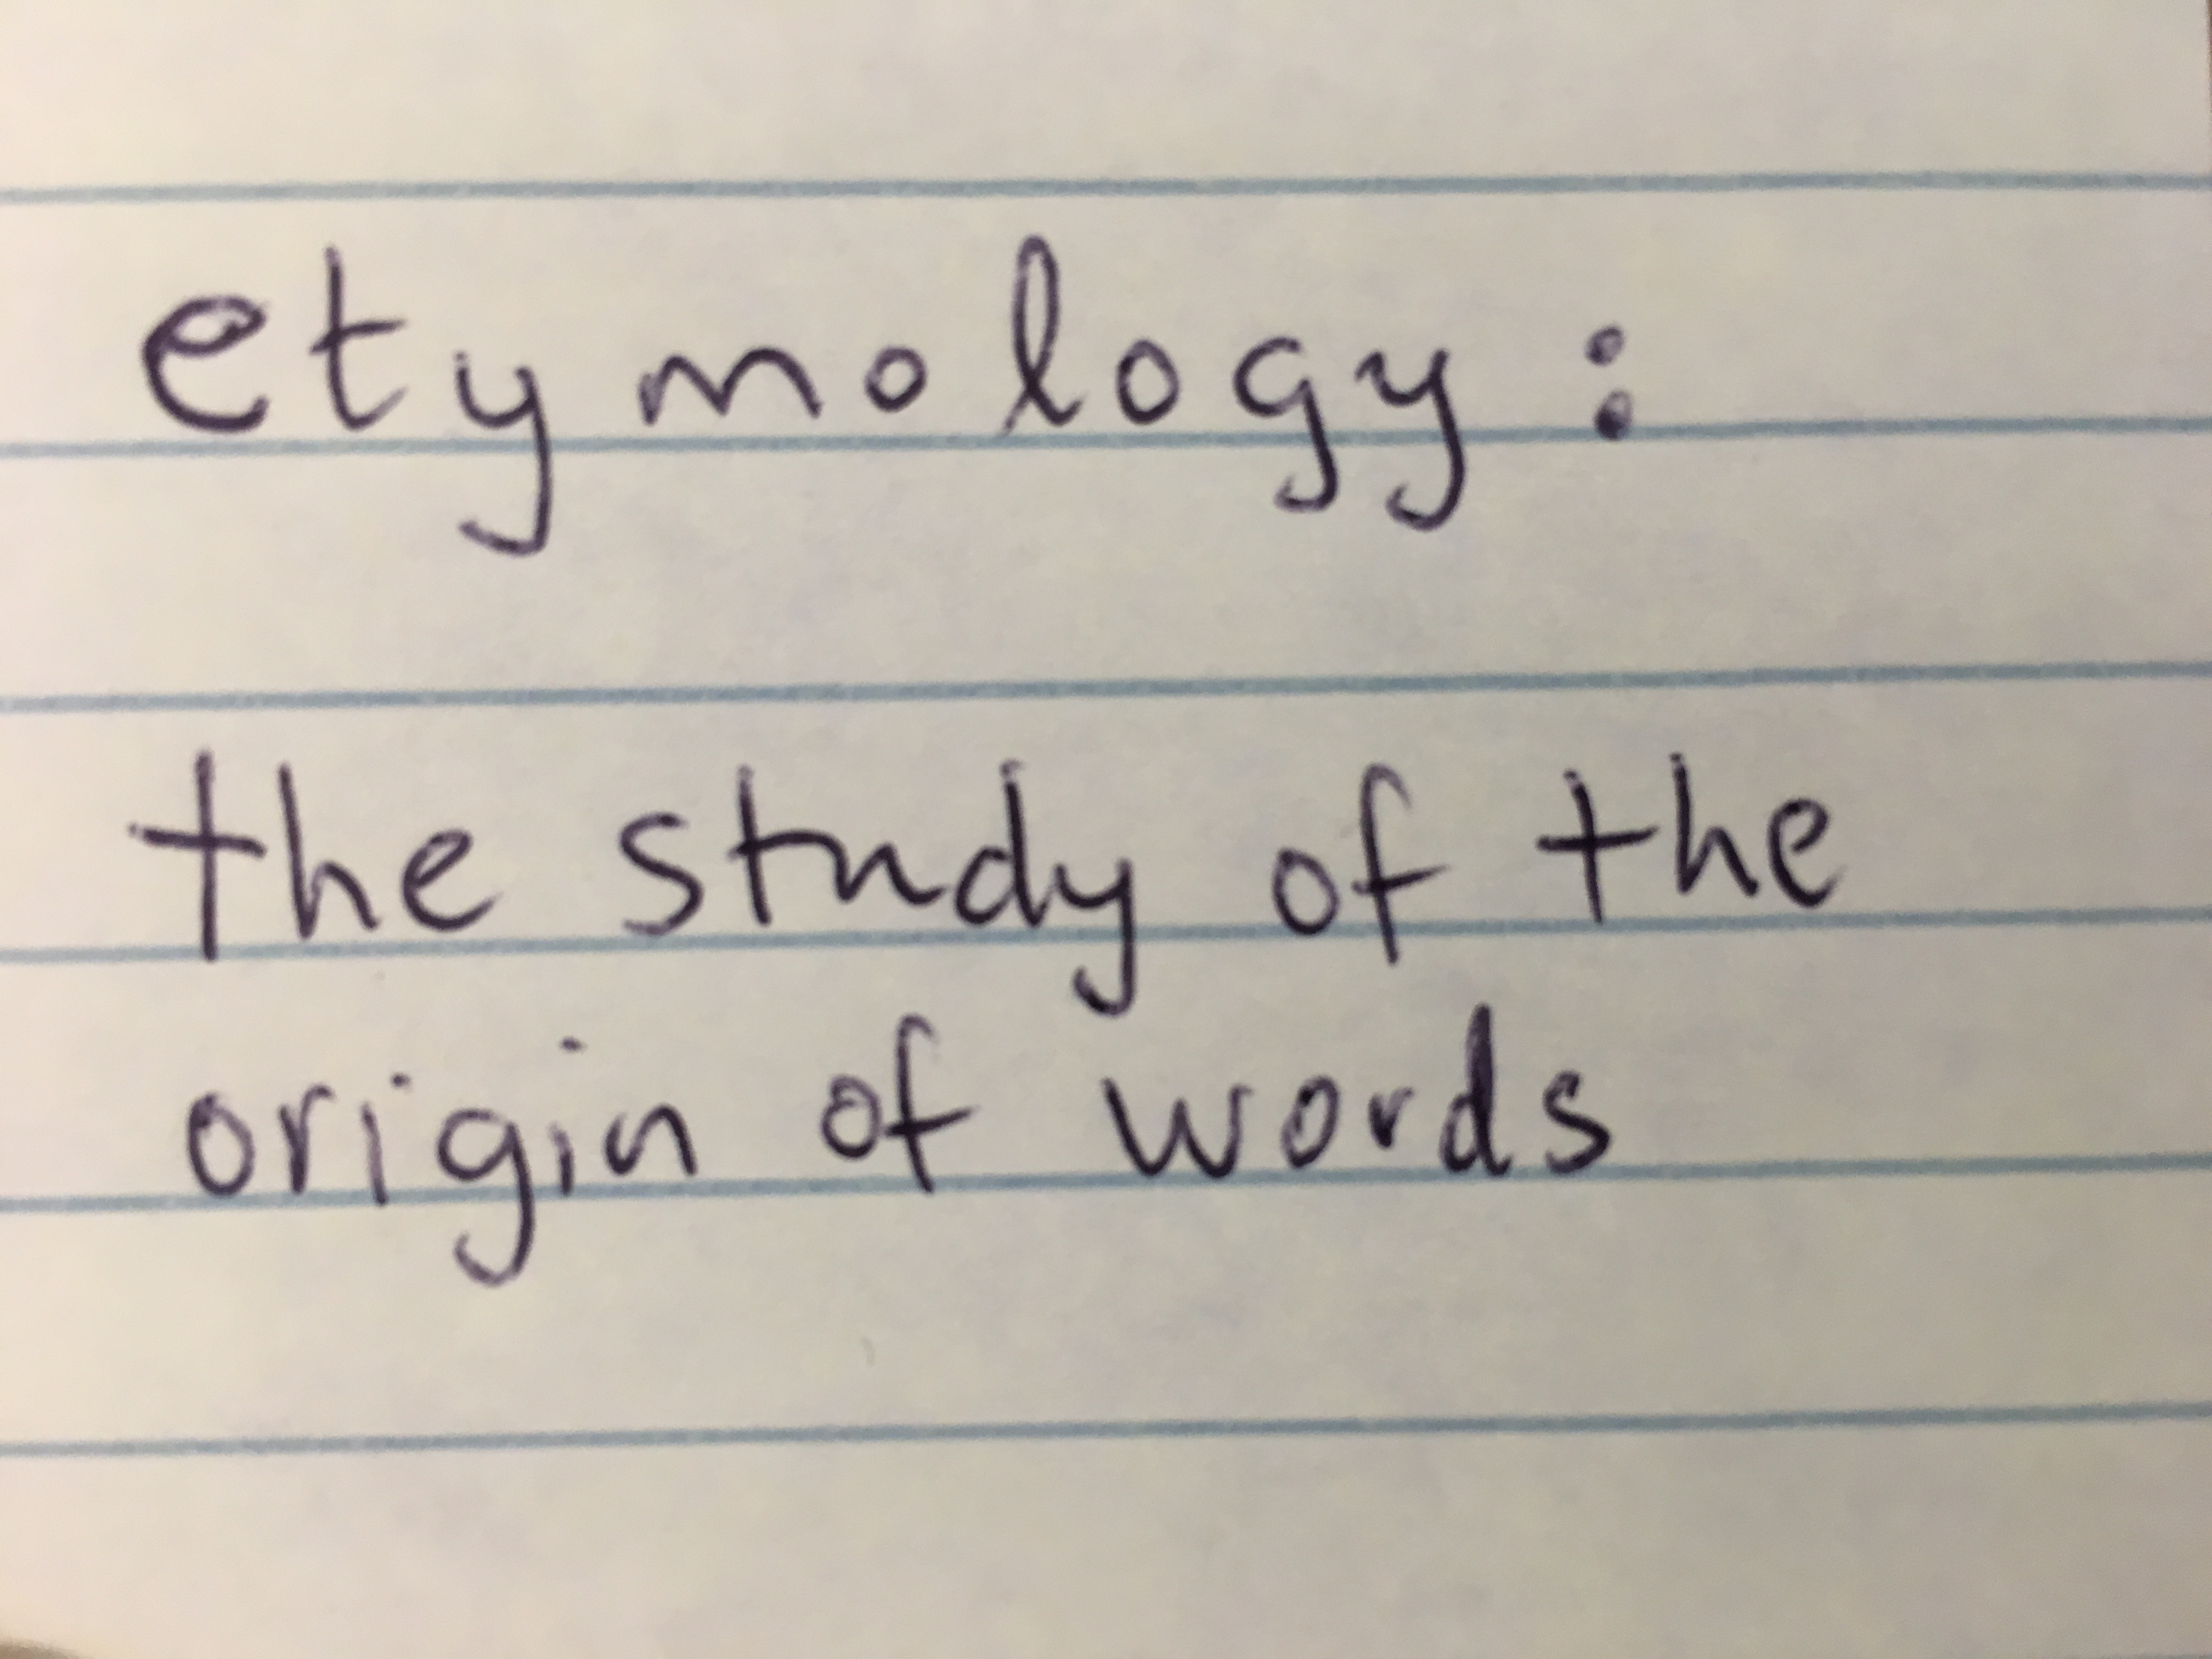
\includegraphics[width=15cm,height=8cm,keepaspectratio]{solution_1d.jpg}
    \caption{assignment-1-d.txt MAC cipher decrypted and decoded jpeg}
  \end{figure}
\end{homeworkProblem}
\end{document}

%%% Local Variables:
%%% mode: latex
%%% TeX-master: t
%%% End: